\begin{frame}[label=title]
    \centering
    \begin{figure}[H]
        
\includegraphics[keepaspectratio, width=0.7\paperwidth, height=\paperheight]{Logos/LeeLogo}
    \end{figure}
    Informatik: Data Science und Sicherheit\\
    \emoji{clamp}\textbf{Kompression}: Intro
\end{frame}

\begin{frame}{Weshalb Kompression? \emoji{clamp}}
	\begin{itemize}
		\item Speicherplatz optimieren
	\end{itemize}
	\begin{figure}[H]
		\centering
		
\includegraphics[width=.6\textwidth]{GrundlagenInfo/04_Kompression/Figures/compression3}
	\end{figure}
	\begin{figure}[H]
		\centering
		\raisebox{-0.5\height}{
\includegraphics[width=.2\textwidth]{GrundlagenInfo/04_Kompression/Figures/compression1}}
		\raisebox{-0.5\height}{$\rightarrow$}
		\raisebox{-0.5\height}{
\includegraphics[width=.25\textwidth]{GrundlagenInfo/04_Kompression/Figures/compression2}}
	\end{figure}
\end{frame}

\begin{frame}{Weshalb Kompression? \emoji{clamp}}
	\begin{itemize}
		\item Speicherplatz optimieren
	\end{itemize}
	\begin{figure}[H]
		\centering
		\raisebox{-0.5\height}{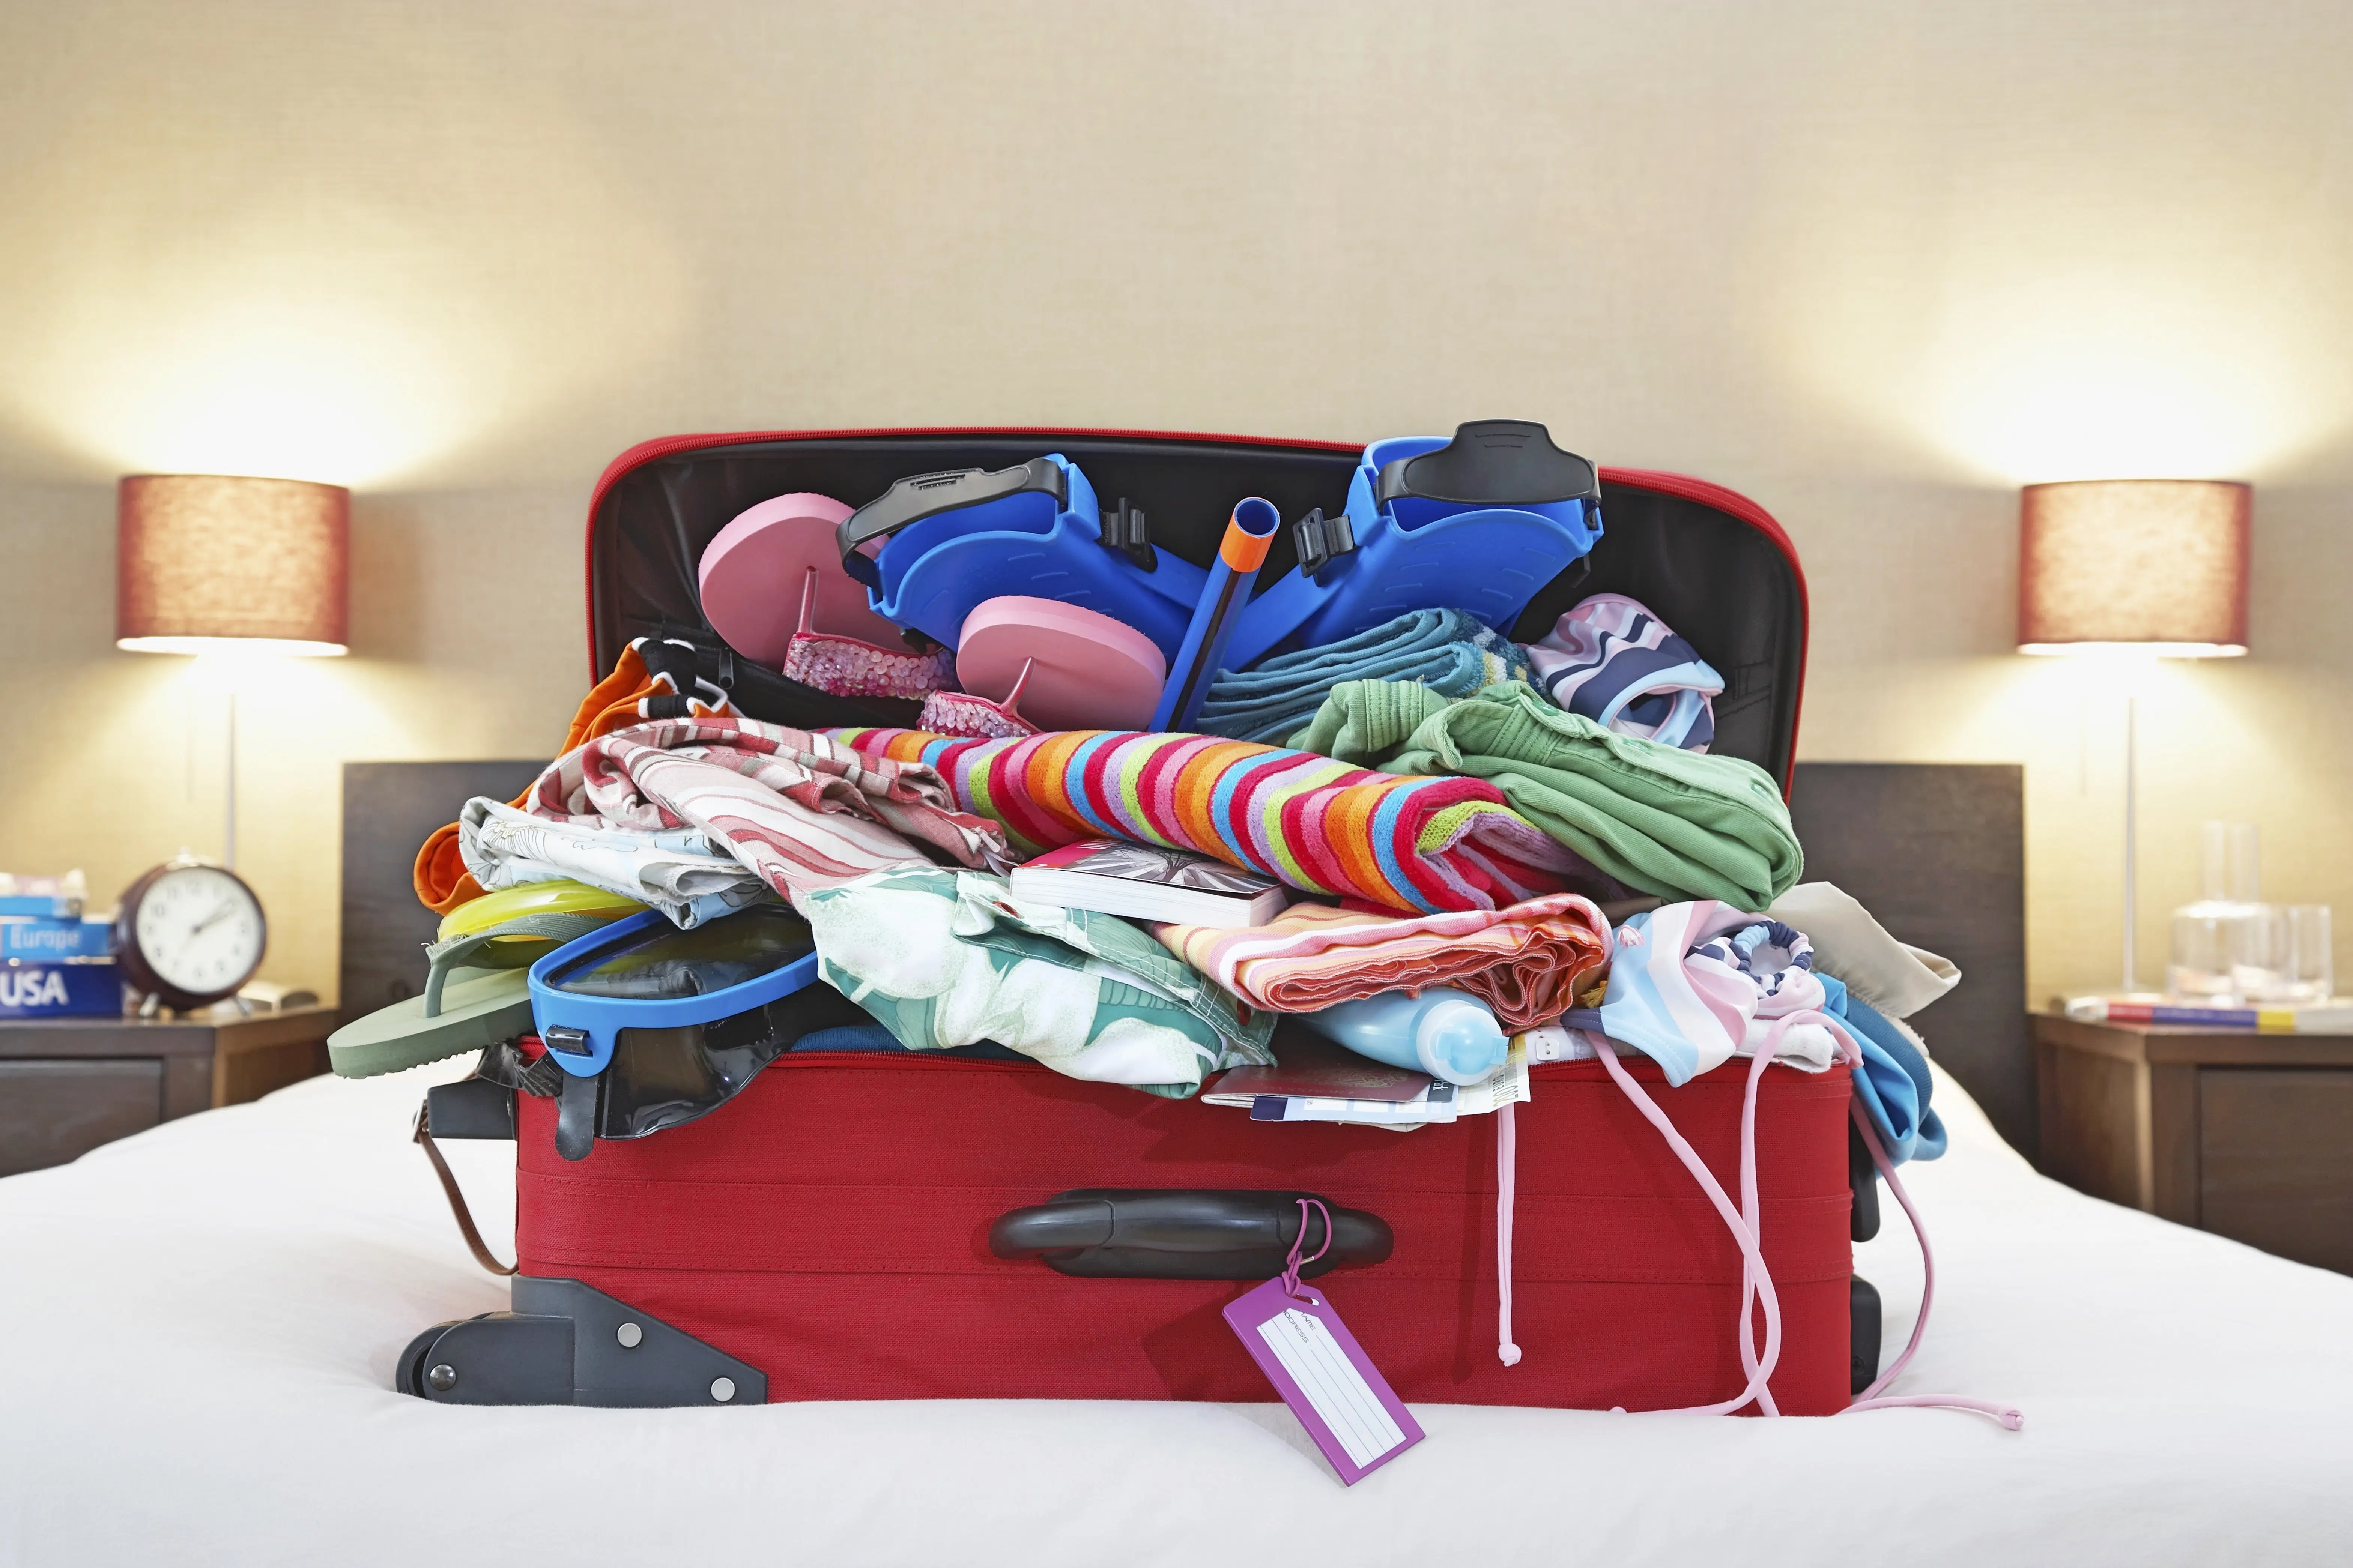
\includegraphics[width=.45\textwidth]{GrundlagenInfo/04_Kompression/Figures/messy_suitcase.jpg}}
		\raisebox{-0.5\height}{$\rightarrow$}
		\raisebox{-0.5\height}{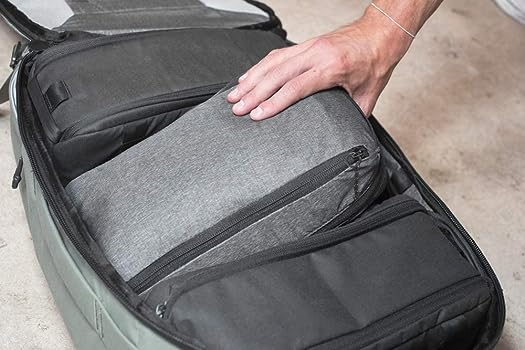
\includegraphics[width=.45\textwidth]{GrundlagenInfo/00_Programmieren/Figures/prog-packing-cubes}}
	\end{figure}
\end{frame}

\begin{frame}{Weshalb Kompression? \emoji{clamp}}
	\begin{itemize}
		\item Speicherplatz optimieren
	\end{itemize}
	\begin{figure}[H]
		\centering
		\raisebox{-0.5\height}{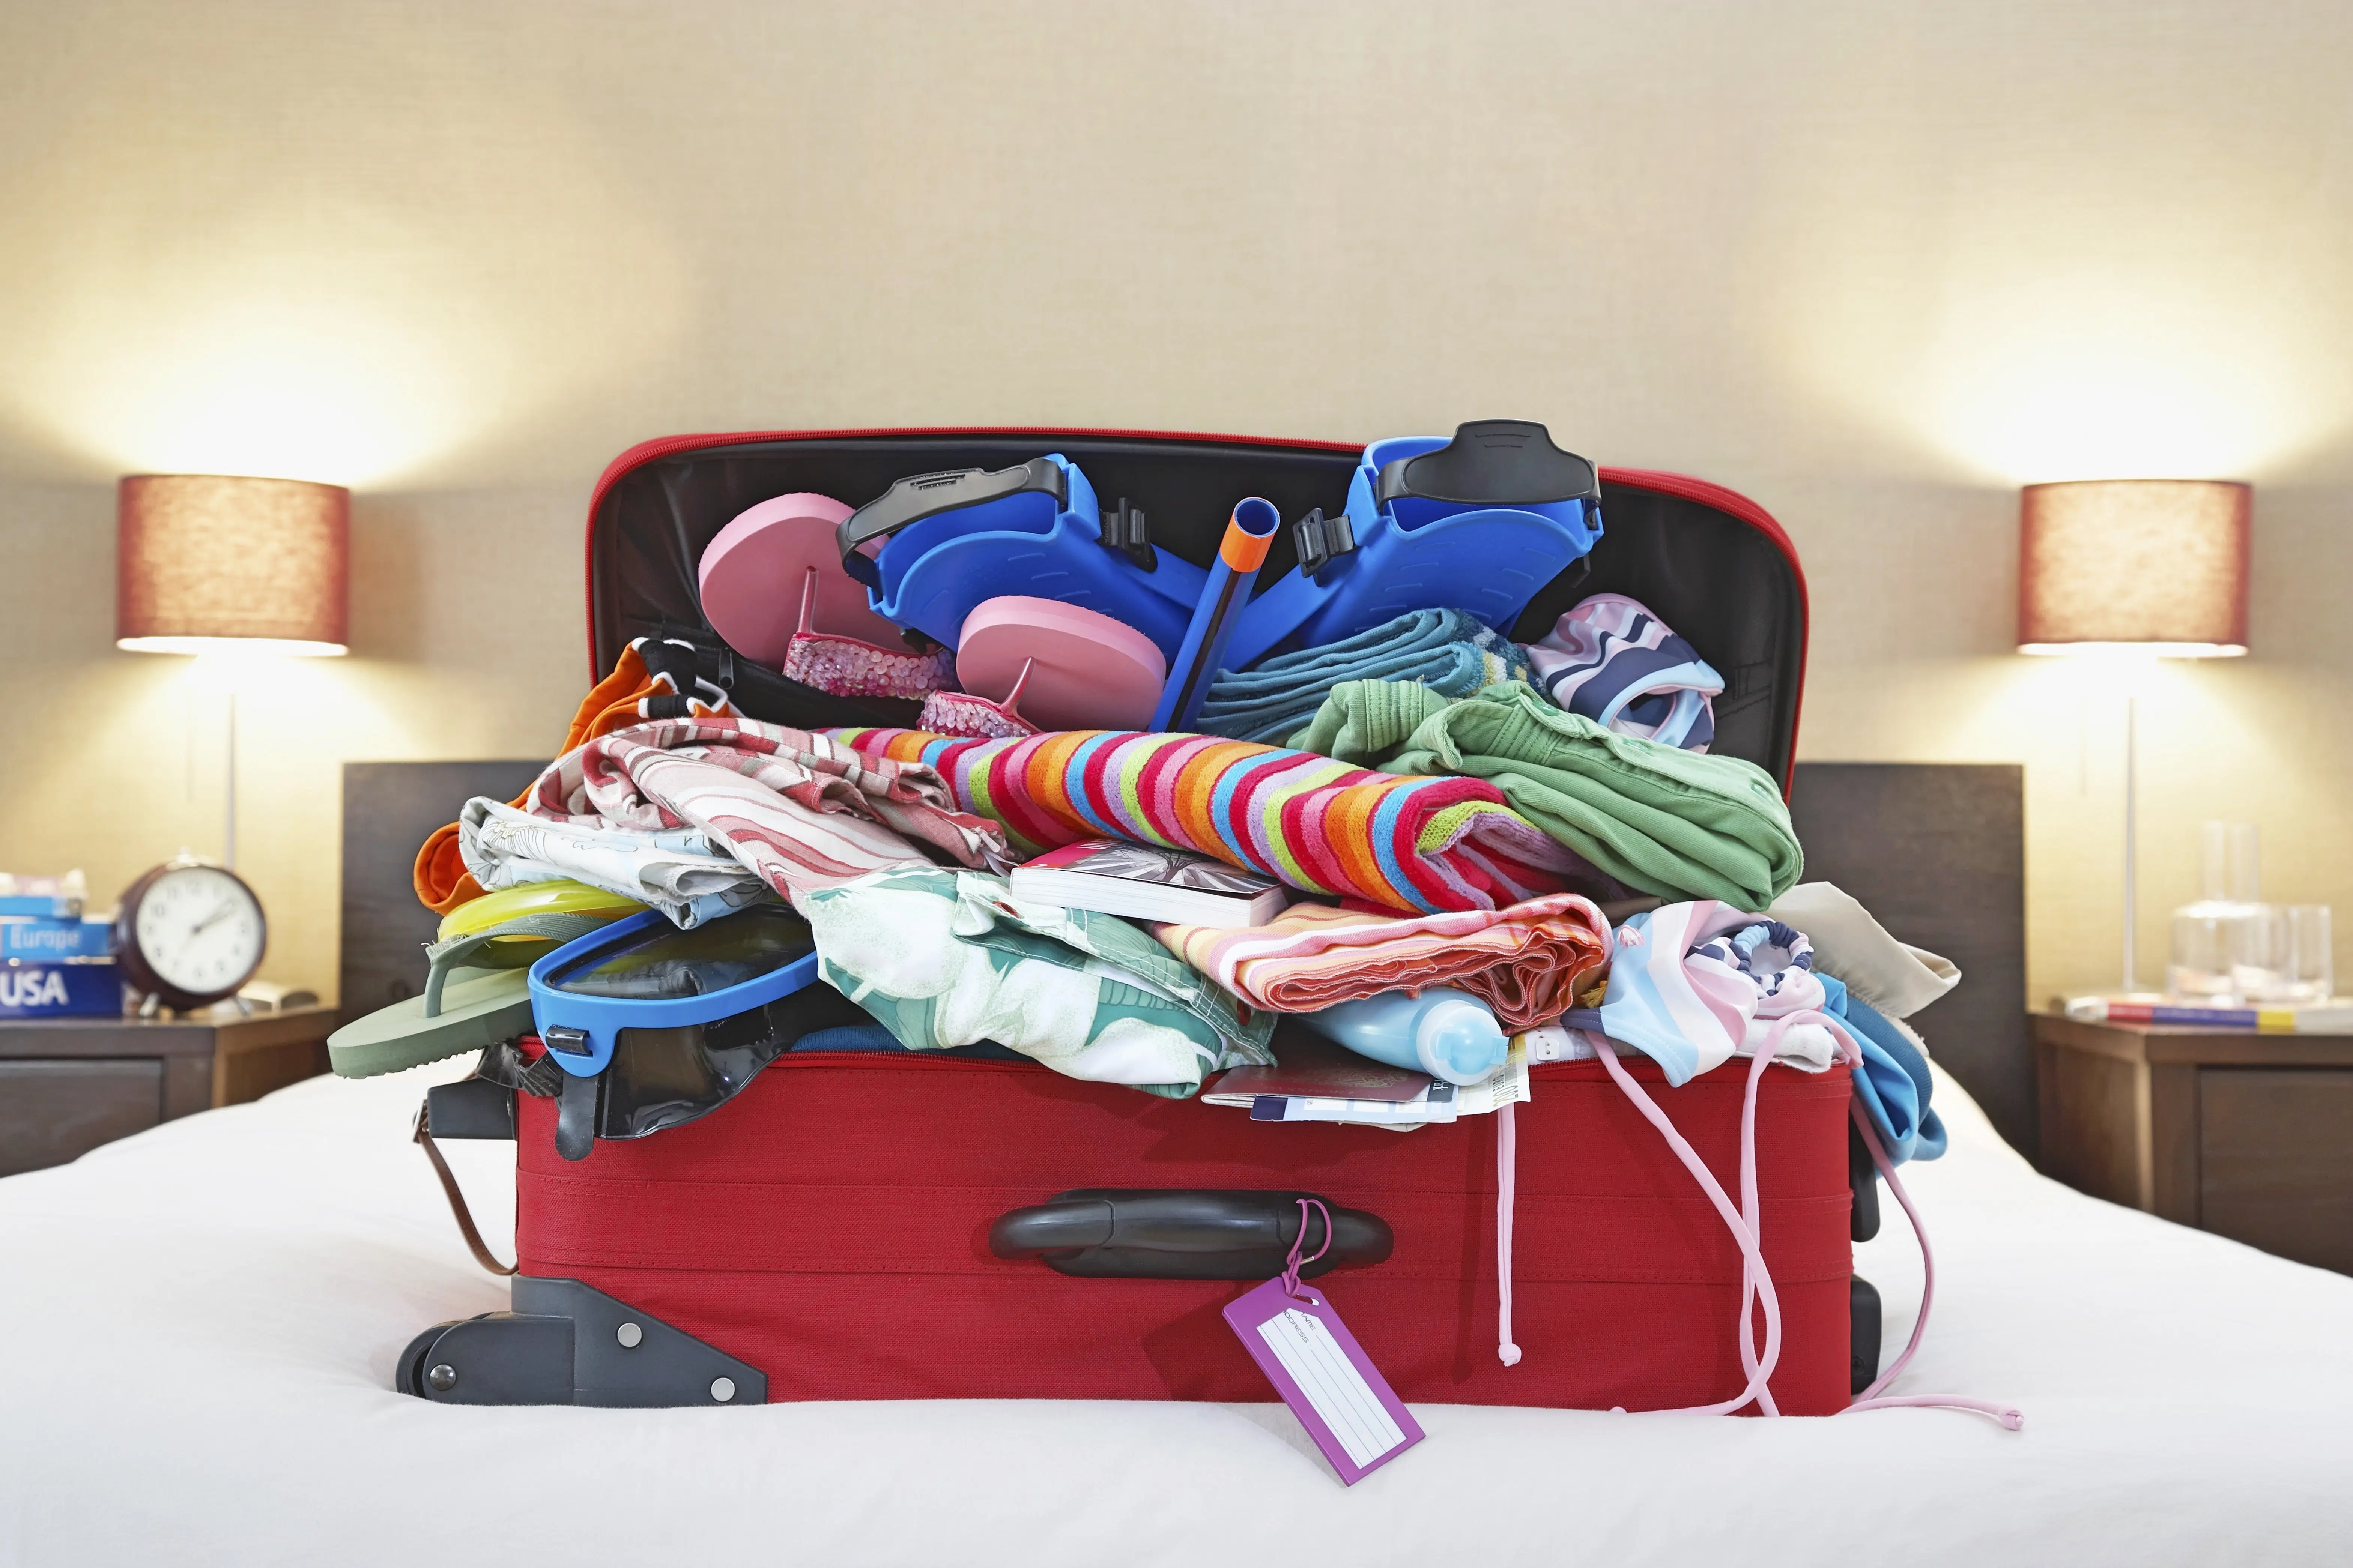
\includegraphics[width=.45\textwidth]{GrundlagenInfo/04_Kompression/Figures/messy_suitcase.jpg}}
		\raisebox{-0.5\height}{$\rightarrow$}
		\raisebox{-0.5\height}{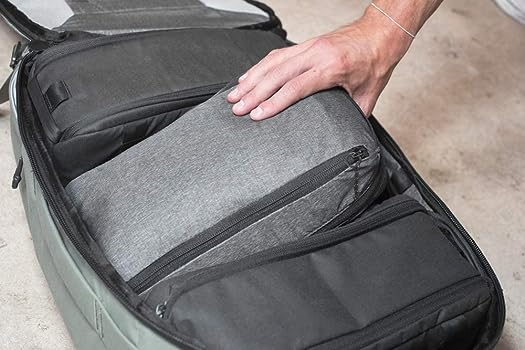
\includegraphics[width=.45\textwidth]{GrundlagenInfo/00_Programmieren/Figures/prog-packing-cubes}}
	\end{figure}
\end{frame}

\begin{frame}{Weshalb Kompression? \emoji{clamp}}
	\begin{itemize}
		\item Wartezeit verkürzen
	\end{itemize}
	\resizebox{!}{.5\height}{%
	\begin{tikzpicture}
		\path[mindmap,concept color=black,text=white]
		node[concept] {Computer}
		[clockwise from=0]
		child[concept color=green!50!black] {
			node[concept] {Computer}
			[clockwise from=90]
			child { node[concept] {Computer} }
			child { node[concept] {Computer} }
			child { node[concept] {Computer} }
			child { node[concept] {Computer} }
		}  
		child[concept color=blue] {
			node[concept] {Computer}
			[clockwise from=-30]
			child { node[concept] {Computer} }
			child { node[concept] {Computer} }
		}
		child[concept color=red] { node[concept] {Computer} }
		child[concept color=orange] { node[concept] {Computer} };
	\end{tikzpicture}}
\end{frame}

\begin{frame}{Verlustfreie vs. verlustbehaftete Kompression}
	Einige Beispiele:
	\begin{table}[H]
		\begin{tabular}{c||c|c}
			\textbf{Anwendung} & \textbf{Verlustfrei} & \textbf{Verlustbehaftet} \\\midrule
			\textbf{Audio} & \texttt{.flac, .aac} & \texttt{.mp3}\\\hline
			\textbf{Dateien} & \texttt{.zip}, \texttt{.rar} & \texttt{-}\\\hline
			\textbf{Video} & \texttt{.raw} & \texttt{.mp4}, \texttt{.avi}, \texttt{.mov} \\\hline
			\textbf{Fotografie} & \texttt{.raw}, \texttt{.psd}, \texttt{.gif} & \texttt{.jpg}, \texttt{.png}\\\hline
			\textbf{Grafik} & \texttt{.svg}, \texttt{.pdf}
		\end{tabular}
	\end{table}


\end{frame}
\begin{frame}{Bilder: Beispiel}
	\begin{figure}
		\centering
		\begin{subfigure}{.45\linewidth}
			\begin{tikzpicture}[boximg]
				\node[anchor=south west] (img) {
\includegraphics[width=\linewidth]{{GrundlagenInfo/04_Kompression/Figures/LeeLogo 300 dpi.jpg}}};
				\begin{scope}[x=(img.south east),y=(img.north west)]
					\node[draw,minimum height=.3cm,minimum width=.75cm] (B1) at (0.48,0.47) {};
				\end{scope}
			\end{tikzpicture}
			\caption{}
		\end{subfigure}\\[0.5\baselineskip]
		\begin{subfigure}{\linewidth}
			\begin{tikzpicture}[boximg]
				\node (img1) {
\includegraphics[width=0.9\linewidth]{GrundlagenInfo/04_Kompression/Figures/LeeLogo 300 dpi zoom}};
				\draw (img1.south west) rectangle (img1.north east);
			\end{tikzpicture}\hfill%
			\caption{}
		\end{subfigure}
		\begin{tikzpicture}[overlay,boximg]
			\draw (B1) -- (img1);
		\end{tikzpicture}
		\caption{\texttt{LeeLogo\textbf{.jpg} (48 KB, 300 dots per inch)}}
	\end{figure}
\end{frame}

\begin{frame}{Bilder: Beispiel}
	\begin{figure}
		\centering
		\begin{subfigure}{.45\linewidth}
			\begin{tikzpicture}[boximg]
				\node[anchor=south west] (img) {
\includegraphics[width=\linewidth]{{GrundlagenInfo/04_Kompression/Figures/LeeLogo.pdf}}};
				\begin{scope}[x=(img.south east),y=(img.north west)]
					\node[draw,minimum height=.3cm,minimum width=.75cm] (B1) at (0.48,0.47) {};
				\end{scope}
			\end{tikzpicture}
			\caption{}
		\end{subfigure}\\[0.5\baselineskip]
		\begin{subfigure}{\linewidth}
			\begin{tikzpicture}[boximg]
				\node (img1) {
\includegraphics[width=0.9\linewidth, clip, trim=115 30 130 30]{GrundlagenInfo/04_Kompression/Figures/LeeLogo.pdf}};
				\draw (img1.south west) rectangle (img1.north east);
			\end{tikzpicture}\hfill%
			\caption{}
		\end{subfigure}
		\begin{tikzpicture}[overlay,boximg]
			\draw (B1) -- (img1);
		\end{tikzpicture}
		\caption{\texttt{LeeLogo\textbf{.pdf}, (28 KB)}}
	\end{figure}
\end{frame}



\begin{frame}{Kompression: Beispiel}
	\centering
	Wie können wir folgenden Text effizient Kodieren?\\[.5cm]
	AACABAAACBACAACADAAD
	
	\begin{table}[H]
		\begin{tabular}{c|c|c|c|c}
			\textbf{Buchstabe} & \textbf{A} & \textbf{B} & \textbf{C} & \textbf{D} \\\midrule\midrule
			Häufigkeit & 12 &  2 & 4 & 2 \\\hline
			Relative Häufigkeit & 60\% & 10\% & 20\% & 10\% \\\hline
			``Naive'' Kodierung: & 00 & 01 & 10 & 11 \\\hline
			``Effiziente'' Kodierung: & 0 & 110  & 10&  111\\
		\end{tabular}
		\only<2>{
		\begin{itemize}
			\item ``Naive'' Codierung (40 Zeichen):\\ \texttt{0000100001000000100100100000100011000011} 
			\item ``Effiziente'' Codierung (32 Zeichen, -20\% Ersparnis):\\ \texttt{0010110000101100100010011100111}\\
		
		\end{itemize}
		}

		\only<3>{
		Beide Codierungen sind \textbf{präfixfrei}: Kein Codewort ist Anfangsstück (Präfix) eines anderen Codeworts}
	\end{table}
\end{frame}

\begin{frame}[fragile]{Codierung als Baumdiagramm}
	\begin{table}[H]
		\centering
			\begin{tabular}{c|c|c|c|c}
			\textbf{Buchstabe} & \textbf{A} & \textbf{B} & \textbf{C} & \textbf{D} \\\midrule\midrule
			Relative Häufigkeit & 60\% & 10\% & 20\% & 10\% \\\hline
			``Effiziente'' Kodierung: & 0 & 110  & 10&  111\\
		\end{tabular}
	\end{table}
	\begin{tikzpicture}
		[-,>=stealth',level distance=15mm,
		level 1/.style={sibling distance=60mm},
		level 2/.style={sibling distance=30mm},
		level 3/.style={sibling distance=15mm},
		level 4/.style={sibling distance=15mm}, leaf/.style={circle, draw}, label/.style={red},edge from parent path={(\tikzparentnode.south) -- (\tikzchildnode)}] 
		
		
		\usetikzlibrary{shapes}
		\tikzstyle{c} = [draw, shape=circle]
		\tikzstyle{n} = [text width=1cm,align=center]
		\tikzstyle{r} = [text=red]
		
		\node[]{}[edge from parent]
		child {node[n] {A\\ \textcolor{red}{0}}
			edge from parent coordinate (ea);
		}
		child {node[]{}
			child {node[text width=1cm,align=center]{C\\ \textcolor{red}{10}}
				edge from parent coordinate (e25);
			}
			child {node[]{}
				child{node[n]{B\\ \textcolor{red}{110}}
					edge from parent coordinate (e14);
				}
				child{node[n]{D \\ \textcolor{red}{111}}
					edge from parent coordinate (e16);
				}
				edge from parent coordinate (e30);
			}
			edge from parent coordinate (e55);
		};
		% code labels
		\node[r] at([yshift=2mm]ea)  {0};
		\node[r] at([yshift=2mm]e55) {1};
		\node[r] at([xshift=-2mm,yshift=2mm]e25) {0};
		\node[r] at([xshift=2mm,yshift=2mm]e30) {1};
		\node[r] at([xshift=-2mm,yshift=1mm]e14) {0};
		\node[r] at([xshift=2mm,yshift=1mm]e16) {1};
	\end{tikzpicture}
\end{frame}

\begin{frame}[label=auftrag]{Auftrag}
	\begin{itemize}
		\item \aufgabebox{Aufgabe 1.1, 1.2}
	\end{itemize}
\end{frame}


\begin{frame}{Appendix}
\end{frame}

\begin{frame}{Kompression: Beispiel}
	\centering
	WENN \emoji{blush} HINTER \emoji{blush} $\triangle$, $\triangle$ EINIGE \emoji{blush} ANDEREN \emoji{blush} NACH.
	
	\only<2>{
		\rule{\linewidth}{.5pt}\\
		\textbf{Auflösung (beispielsweise)}:\\
		WENN GRIECHEN HINTER GRIECHEN RENNEN, RENNEN EINIGE GRIECHEN ANDEREN GRIECHEN NACH.
	}
\end{frame}


\begin{frame}{Kompression: Beispiel}
	\centering
	WENN KLEINE BIENEN HINTER GROSSEN \#3 FLIEGEN, \#1 \#7 \#4 \#6 \#2 NACH.
	\only<2>{
		\rule{\linewidth}{.5pt}\\
		\textbf{Auflösung}:\\
		WENN KLEINE BIENEN HINTER GROSSEN BIENE FLIEGEN, FLIEGEN KLEINE BIENEN GROSSEN BIENEN NACH.
	}
\end{frame}


\begin{frame}{Kompression: Beispiel}{Römer \emoji{amphora}}
\begin{itemize}
	\item Leder und Stein: Teure Materialien
	\item Römische Zahlendarstellung: z.B. Zahl \textbf{999}
	\begin{center}
		\texttt{CCCCCCCCCXXXXXXXXXIIIIIIIII}\\
		$\downarrow$\\
		Erfindung der Ziffern D (500), L (50), V(5)\\
		$\downarrow$\\
		\texttt{DCCCCLXXXXVIIII} \\
		$\downarrow$\\
		Effizientere Schreibweise\\
		$\downarrow$\\
		IM
	\end{center}
\end{itemize}
\end{frame}